\chapter{Heat Modeling of Integrated Devices}
\label{ch:heatmodeling}
\section{Heat Models using physical device models}
\subsection{Other Methods}
\subsubsection{RC-\,Networks}
\section{Extension to On-Line Evolution of Heat Models}

\section{Temperature Measurement Methods}

\subsection{Built-In Temperature Sensor}
\label{sec:diode}
The most common way to measure temperatures on a \ac{VLSI} chip is to implement a temperature sensor in \ac{CMOS}. As stated in \cite{Bakker1996} the most effective way to achieve this goal is by using vertical bipolar transistors. This approach exploits the fact that the base-emitter voltage $V_{be}$ of a bipolar transistor decreases approximately by $2\,mV\symbol{23}^{\circ}C$ and hence almost linearly with the temperature. 
Furthermore, the difference between two measured base-emitter voltages $\delta V_{be}$ is almost linearly proportional to the absolute temperature $T_{abs}$ (ptat) and can be expressed as depicted in Equation~\ref{eq:PTAT}.

\begin{equation}
\label{eq:PTAT}
V_{ptat}(T_{abs}) = \frac{kT}{q}\cdot ln(p)
\end{equation}

The parameters for Equation~\ref{math:PTAT} are the following:

\begin{itemize}
	\item Boltzman's constant, $k = 1.38 \times 10^{-23}$
	\item Temperature in Kelvin, $T [\symbol{23}^{\circ}\,K]$
	\item Charge on an electron in coulomb, $q = 1.6 \times 10^{-19}\,C$
	\item Emission current density ratio $p$
\end{itemize}

This temperature sensor achieves an accuracy of $\pm1\symbol{23}^{\circ}C$, by calibrating $V_{be}$ at room temperature \cite{Bakkar1996}.

Also in modern \acp{FPGA} there is a trend of providing a pre-calibrated thermal diode, which are also provided at \ac{CMOS} level. These devices can for example be found at the Virtex-5 \ac{FPGA} by Xilinx, where the proportionality between the voltage and die temperature is as well exploited. Xilinx specifies this correlation with Equation~\ref{eq:XIL_PTAT} \cite{Xilinx2011a}.

\begin{equation}
\label{eq:XIL_PTAT}
V_{ptat}(T_{abs}) = 10 \cdot \frac{kT_{abs}}{q}\cdot ln(10)
\end{equation}

Note that the emission current density ratio is here set to $p = 10$. Hence, temperature coefficient of $V_{ptat}$ is $-2\,mV/\symbol{23}^{\circ}C$.

Since the thermal diode is pre-calibrated, the temperature can be derived as depicted in Equation~\ref{eq:tempcalc}. To allow the further calculation it is mandatory to convert $V_{ptat}$, given as analog signal, into a digital number. The thermal diode on a Virtex-5 \ac{FPGA} digitizes $V_{abs}$ with the help of the built-in \ac{ADC} and produces the 10\,bit output \ac{ADC} code $V_ADC$. The resulting maximum-measurement error of this on-chip temperature sensor is specified with $\symbol{23}^{\circ}C$ \cite{Xilinx2011a}.

\begin{equation}
\label{eq:tempcalc}
	T[\symbol{23}^{\circ}C] = \frac{V_{ADC}\times 503.957}{1024} - 273.15
\end{equation}

\subsection{Infrared Cameras}
\label{sec:IRC}
Besides the above-named on-chip solutions of measuring the internal temperature, there is also the possibility to use \ac{IR} cameras. 

For instance, \cite{Ebi2011} measured a spatial thermal gradient of 2\symbol{23}$^{\circ}C$ over 10\,mm on a Xilinx Virtex II \ac{FPGA} using an infrared camera.
Furthermore \cite{Agne2013}.

Shortcomings of this approach are that one always needs direct view on the chip's silicon layer \cite{Lopez-Buedo2004}. I.e. no heat sink, package or other material, where the emission cannot be determined.
Besides the high price for these devices, \ac{IR} cameras cannot be employed in actual working conditions, because of their size \cite{Nowroz2011}.


\begin{figure}[h]
		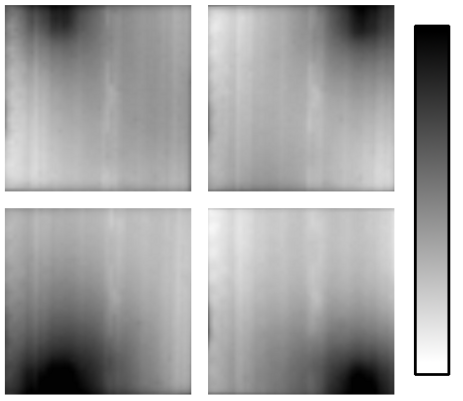
\includegraphics[width=\textwidth]{__pics/infra_heater}
		\caption{Four infrared images of the \ac{FPGA} with temperatures from 80\symbol{23}$^{\circ}C$ (white) to 95\symbol{23}$^{\circ}C$ (black) cf. \cite{Agne2013}}
		\label{pic:heater_infrared}	
	\end{figure} 

\subsection{Ring Oscillators}

Nowadays, a widely spread technique to measure the internal on-chip temperatures of \ac{FPGA}-based systems are based on \acp{RO}. These devices are composed of an odd number of inverters, which are connected in a chain. The endmost inverter's output is fed back to the first inverter. Figure~\ref{pic:simple_ro} depicts such a basic \ac{RO}. This leads to a device without a stable condition, causing each inverter's output to oscillate, i.\,e. the output $Q$ toggles between $0$ and $1$ and maximum speed with frequency $f_{osc}$. A longer inverter chain leads to a lower frequency and in addition to less power consumption \cite{Velusamy2005}.
It is because of the fact that the \ac{RO}'s frequency $f_{osc}$ is inversely proportinal to the on-chip temperature \cite{Lopez-Buedo2002}, that \acp{RO} can be used to measure the temperature on any location on the \ac{FPGA}. The output frequency $f_{osc}$ is dependant on the curcuit's delay. Furthermore, it is also known that \acp{RO} can be used in order to measure delay, leakage and dynamic power \cite{Zick2012}. 

\begin{figure}[h]
		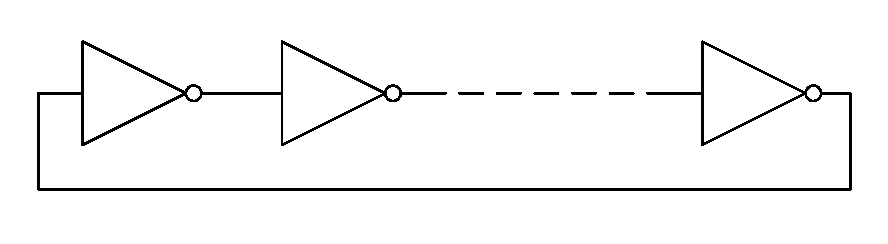
\includegraphics[width=\textwidth]{__pics/RO.pdf}
		\caption{A basic Ring Oscillator, consisting of an odd number of inverters}
		\label{pic:simple_ro}	
	\end{figure} 

\subsubsection{Methodology}

Measuring the internal on-chip temperature necessarily requires knowledge about the frequency $f_{osc}$ of the \ac{RO}. In order to estimate the frequency, several approaches \cite{Sayed2011, Lopez-Buedo2002, Velusamy2005, Happe} make use of \acp{RO} combined with a capture counter. The counter, as depicted in Figure~\ref{pic:Temp_Sensor}, is clocked with a system \ac{CLK} and by the oscillating output $Q$ of the \ac{RO}. $Q'$ toggles at the speed of $Q$ and is sampled by \ac{CLK}. Put simply, the capture counter samples the number $S$ of oscillations at the signal $Q'$ with the frequency $clk$. Afterwards the sampled number of oscillations can be derived to $f_{osc}$. 

\begin{figure}[h]
		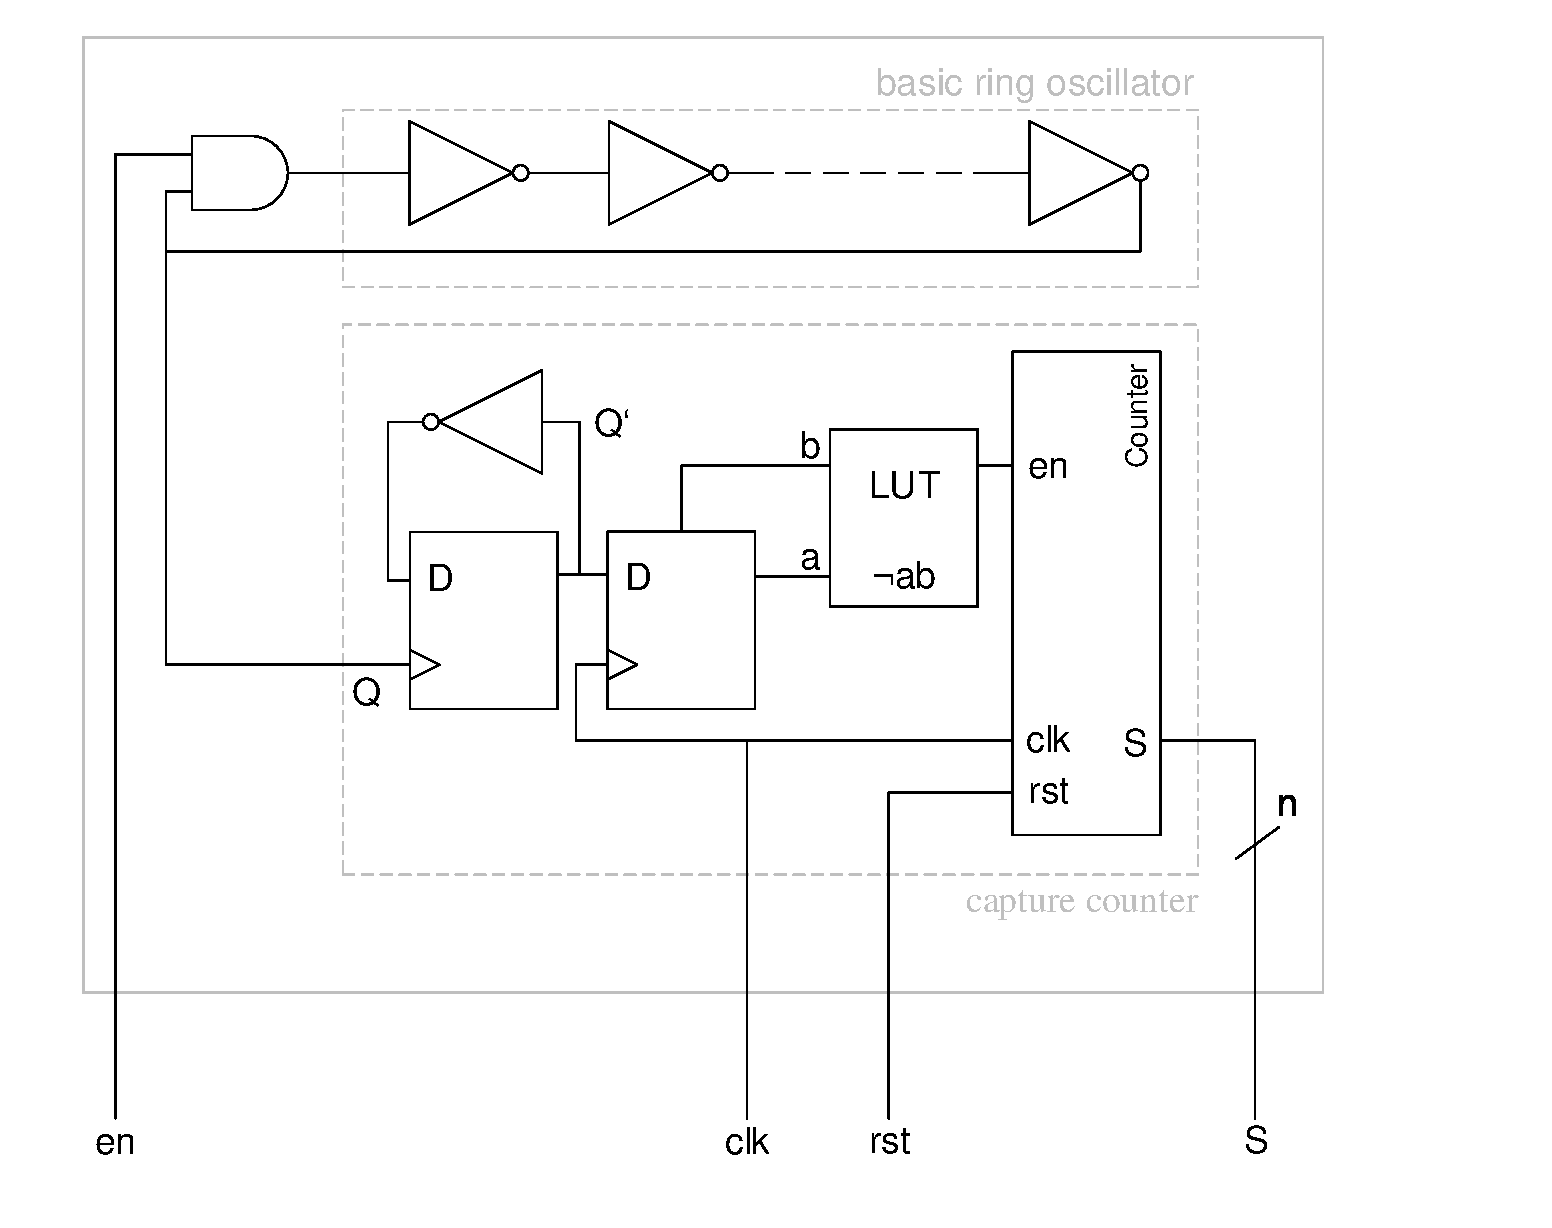
\includegraphics[width=1.15\textwidth]{__pics/Temp_Sensor.pdf}
		\caption{Simplified schematic of a temperature sensor with capture counter cf. \cite{Ruthing2012}}
		\label{pic:Temp_Sensor}	
	\end{figure} 
	
However, there are also differences in implementing the \ac{RO}-based temperature sensor. These variable parameters are: number of inverters, system routing, length of measurement period $t_m$ and the possible use of latches between the inverters. 
The use of latches was proposed in order to minimize the impact of routing \cite{Zick2012}. For \acp{FPGA} designs, it is advisable to use latches instead of the additional wiring between the inverters. 

The benefits of designing on an \ac{FPGA} are the reconfigurability. This possible due to the \acp{CLB} of which the \ac{FPGA} is composed. The \ac{CLB} however comprises slices, which contain \acp{LUT} and \acp{FF}. 
Hence, by using \acp{LUT} for the \ac{RO}'s inverters, the \acp{FF} can be used as latches without significant additional wiring.

In contrast to previous approaches, which used seven \cite{Happe} or eleven inverters \cite{Lopez-Buedo2002, Velusamy2005} and no latches, a high-performance \ac{RO}-based temperature sensor comprises 23 inverters and 24 latches \cite{Ruthing2012}. The quality of the \ac{RO} is derived by sensor resolution and sensor noise/deviation.
In addition to the utilization, the optimal measurement period $t_m$ should not exceed the maximum length of $2^{16}$ clock cycles, which is $655\,\mu s$, when the counter samples with 100\,MHz. For longer measurement periods, there is a risk of self-heating, since \acp{RO} may lead to considerable temperature gradients \cite{Agne2013}.

As previously pointed out, the optimal measurement with the proposed temperature sensor includes the following steps \cite{Ruthing2012}:

\begin{itemize}
	\item Enable \ac{RO} with 23 inverters and 24 latches
  \item Wait $2^{12}$ -- $2^{16}$ clock cycles so that the \ac{RO} can gain a constant frequency
  \item Sample $Q'$ for $t_m$ clock cycles
  \item Disable the \ac{RO}
  \item Read out the counter value $S$.
\end{itemize}

\subsubsection{Calibration Methods}

Given the sensor count $S$ of \ac{RO}-based temperature sensors, it is not possible to predict a function that maps $S$ to a temperature $T$. Instead, the sensors need to be calibrated with an pre-calibrated device, such as the built-in thermal diode, a temperature-controlled oven or an \ac{IR} camera. 
While the device is heated up and cooled down afterwards, $S$ is counted and the temperature is read in regular time intervals. For each sensor placed on the chip the linear mapping function is then determined by partial regression \cite{Lopez-Buedo2002, Ruthing2012}. 

The following approaches request for a temporal temperature gradients equally distributed on the chip. Section~\ref{sec:tempgen} will give an overview of most common and useful methods for heating up the sensors, e.g. the \ac{RO}-based temperature sensors.

As proposed in \cite{Lopez-Buedo2002} the sensors were calibrated by an iron-constantan (Fe-CuNi) thermocouple which is placed in the center of the package exactly measure the on-chip temperature $T$.

Section~\ref{sec:IRC} already illustrated that \ac{IR} cameras are able to exactly measure the on-chip temperature $T$ \cite{Nowroz2011}, provided that the camera is pointing directly on the silicon and the emission value is known. Additionally of course, they can be used for calibrating the \ac{RO}-based temperature sensors with high accuracy. 
WIE GENAU???

Another way to calibrate the sensors is to make use of the built-in thermal diode, which was presented in Section~\ref{sec:diode}. While heating up the chip, the sensor data $S$ and the diode temperature $T_{diode}$ are captured. Again, note that this diode has a $\pm 4�C$ inaccuracy and it is known where the sensor is exactly placed on the \ac{FPGA}.

\subsection{Discussion on Accuracy}
table?
-  +4�C diode (where? no hot spot detection)
-  ROTS (calibrated with +4�C acc and where?!)
-  IR Cam (expensive, no usage in field, silicon view, knowledge about emission)

\section{Temperature Generation Methods}
\label{sec:tempgen}

As said earlier \ac{RO} temperature sensors have to be calibrated before use. For example, this can be done by 
There are several approaches\cite{Velusamy2005, Lopez-Buedo2002, Zick2010}

Several approaches are using a temperature-controlled oven in order to heat up the chip \cite{Velusamy2005, Lopez-Buedo2002, Zick2010}. Either the sensors are calibrated by surrounding temperature or 

	VCC and temperature proportionally ! \cite{Ruthing2012}